\chapter{The Futhark \csharp{} backend}

\begin{figure}[h]
  \centering
  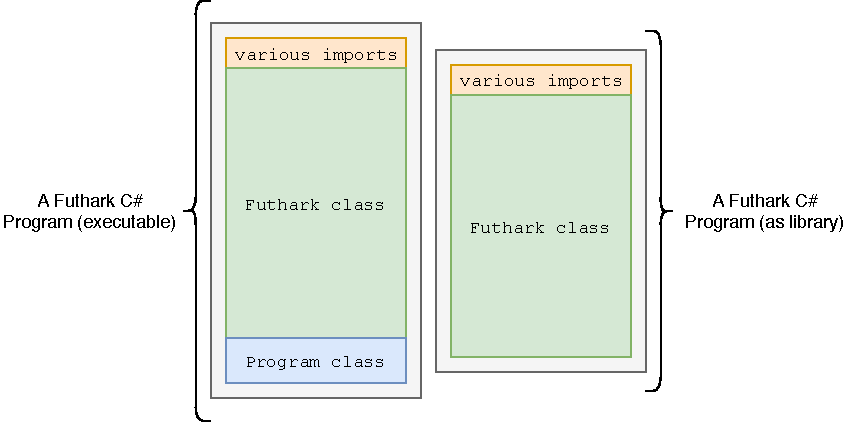
\includegraphics[scale=0.85]{chapters/figs/csharp/futharkcs_wide.pdf}
  \caption{The two possible types Futhark \csharp{} programs}
  \label{fig:futharkcsclasses}
\end{figure}

To be able to use Futhark with \fsharp{} programs, it was necessary to compile
Futhark programs to a language that \fsharp{} could work with.
Although the difference between running a compiled Futhark C- and \csharp{}
executable from the command line is negliable, a Futhark \csharp{} backend would
allow .NET projects to use Futhark libraries natively, instead of running their
Futhark calculations through seperate C or Python modules.

Because \fsharp{} has almost frictionless interoperability with \csharp{}, and \csharp{}s
imperative constructs are very close to the intermediate code that Futhark
generates for it's code generation, it was an easy decision to implement a
\csharp{} generating backend for Futhark, to accompany the already existing C-
and Python backends.

A Futhark backend must be able to do two different programs from a given Futhark
program:

First, it must be able to generate standalone executables which can take input data from the \texttt{stdin} stream, and send
the results to the \texttt{stdout} stream. Although a Futhark C, -Python or
\csharp{} executable should have equivalent functionality, their performance may
vary, and the users may alter between the versions depending on which platforms
that are available on their systems.

Second, and more interesting, it must be able to generate single file libraries
which can then be imported and used in other C, Python or \csharp{} projects, in
the same manner as any other library.

\begin{figure}[h]
  \centering
    \begin{lstlisting}[language=Futhark]
      let main (xs : []i32) : []i32 = map (+2) xs
    \end{lstlisting}
  \caption{A very small Futhark program \texttt{map2.fut}}
  \label{fig:smallfut}
\end{figure}
In example, if we compile the Futhark program in figure \ref{fig:smallfut} as a
Python library, we will be able to use it in a Python program, as showed in figure \ref{fig:smallpython}.
Likewise, we would like to be able to do the same thing in a \csharp{} or an
\fsharp{} context.
\begin{figure}[h]
  \centering
    \begin{lstlisting}[language=python]
      import numpy as np
      from map2 import map2

      xs = np.array([1,2,3])
      map2object = map2()
      xs_res = map2object.map2(xs)
      print xs_res # prints [3,4,5]
    \end{lstlisting}
  \caption{A very small Python program}
  \label{fig:smallpython}
\end{figure}

\subsection{The anatomy of a Futhark \csharp{} program}
\begin{figure}[h]
  \centering
  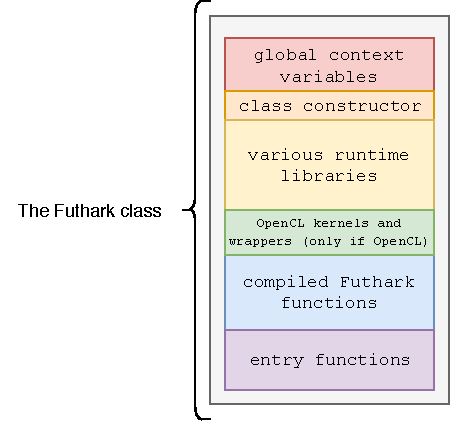
\includegraphics{chapters/figs/csharp/futhark_class.pdf}
  \caption{The layout of the \csharp{} Futhark class}
  \label{fig:futharkclass}
\end{figure}

\begin{figure}[h]
  \centering
  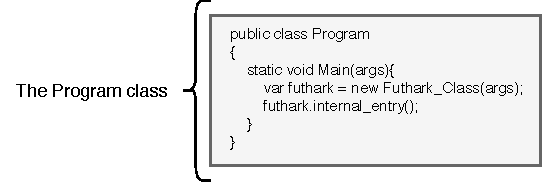
\includegraphics{chapters/figs/csharp/program_class.pdf}
  \caption{The \fshark{} compilation pipeline}
  \label{fig:programclass}
\end{figure}

Designing a Futhark backend for some target language $lang$ is comprised of (mainly) NNNNNN subtasks:
\begin{itemize}
\item Writing a compiler which takes a program written in Futharks
  intermediate language, and expresses them as $lang$ code.
  This compiler covers both ``regular'' $lang$ Futhark programs, but also OpenCL
  powered ones.
  (måske mere uddybende)
  This part takes care of the 

\item Designing the boiler
\end{itemize}


%% DESCRIBE THE DIFFERENCES BETWEEN C# AND THE REST
THE PYTHON BACKEND HAS MUCH FUNCTIONALITY ENCAPSULATED IN PYOPENCL, AND DOESN'T
NEED TO DECLARE VARIABLES BEFORE SETTING THEM
LESS COMPLEX GENERATOR NEEDED AS VARIOUS OPENCL STATEMENTS ARE HANDLED
AUTOMATICALLY BY LIBRARY

C BACKEND MUST BE AWARE OF ALL SIZES AND EVERYTHING AT COMPILE TIME, WHICH MEANS
STATES MUST BE ALLOCATED THROUGH COMPLEX STRUCTS AT COMPILE TIME, AND STRUCTS
MUST BE DEFINED AT COMPILE TIME AS WELL

CSHARP GENERATOR IS SOMEWHERE INBETWEEN AS IT IS CAN HANDLE OBJECTS WHICH CAN
CARRY STATE, FURTHERMORE DYNAMIC MEMORY ALLOCATION

% THE DIFFERENCES BETWEEN MEMORY HANDLING IN CS AND CSOPENCL
%% PERFORMANCE ISSUES WITH CS MANAGED ARRAYS

% COMPILING A FUTHARK CS PROGRAM
% USAGE OF A COMPILED FUTHARK CS PROGRAM

% WHY THIS DESIGN

% PERFORMANCE OF FUTHARK-CS AND FUTHARK-CSOPENCL
%% FOR CS-OPENCL, PERFORMANCE IS COMPARABLE TO C-OPENCL
%% FOR CS, PERFORMANCE IS VASTLY INFERIOR TO TO C
%%% WHY IS THAT???????????




%discussion:
% why are we using Cloo, and not other \csharp{} opencl libs
% if Cloo dies, we can achieve similar functioality by writing our own opencl
% lib, as we only uses the bindings from Cloo

% why use \csharp{} when \fshark{} is for \fsharp{}? ImpCode is often directly
% translatable to \csharp{}


%%% Local Variables:
%%% mode: latex
%%% TeX-master: "../thesis"
%%% End: